% Source: Code/xband-radar-sim/docs/radar_simulation_technical.tex
% Description: Matched filter output showing sinc function. Main lobe width equals range resolution. First sidelobe at -13.2 dB without windowing.

\documentclass[border=4pt]{standalone}
\usepackage{algpseudocode}
\usepackage{amsmath,amssymb,amsfonts}
\usepackage[T1]{fontenc}
\usepackage{graphicx}
\usepackage{pgfplots}
\usepackage{tikz}
\usepackage{xcolor}
\pgfplotsset{compat=1.18}
\usetikzlibrary{arrows.meta,positioning,shapes.geometric,calc,patterns,decorations.pathmorphing,3d,angles,quotes}

\definecolor{radargreen}{RGB}{0,255,0}
\definecolor{raycolor}{RGB}{255,165,0}
\definecolor{targetcolor}{RGB}{255,0,0}
\definecolor{groundcolor}{RGB}{139,90,43}
\definecolor{skycolor}{RGB}{135,206,235}
\definecolor{beamcolor}{RGB}{255,255,0}


\begin{document}
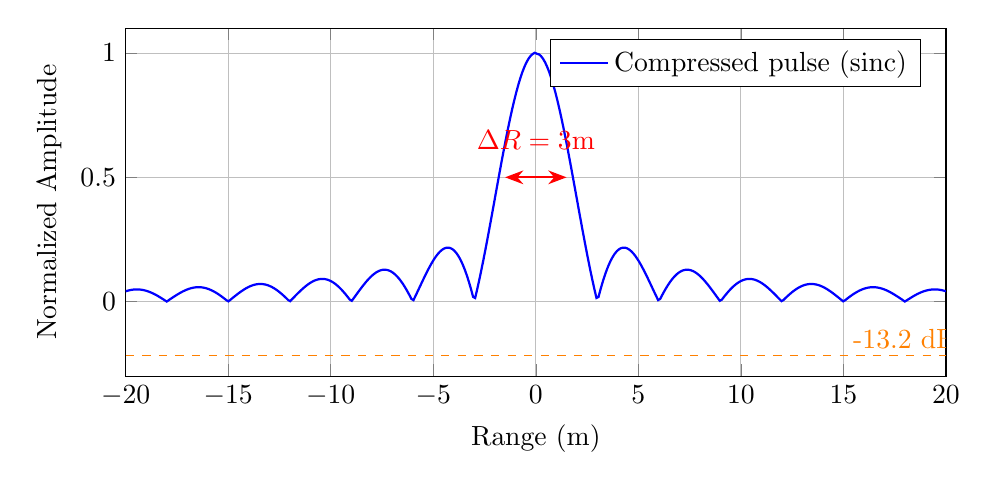
\begin{tikzpicture}
\begin{axis}[
    width=12cm, height=6cm,
    xlabel={Range (m)},
    ylabel={Normalized Amplitude},
    xmin=-20, xmax=20,
    ymin=-0.3, ymax=1.1,
    grid=both,
    legend pos=north east
]
    % Sinc function
    \addplot[thick, blue, domain=-20:20, samples=400] {
        abs(sin(deg(pi*x/3))/(pi*x/3 + 0.0001))
    };
    \addlegendentry{Compressed pulse (sinc)}

    % Main lobe width
    \draw[{Stealth}-{Stealth}, thick, red] (axis cs:-1.5,0.5) -- (axis cs:1.5,0.5);
    \node[red] at (axis cs:0,0.65) {$\Delta R = 3$m};

    % Sidelobe level
    \draw[dashed, orange] (axis cs:-20,-0.217) -- (axis cs:20,-0.217);
    \node[orange, right] at (axis cs:15,-0.15) {-13.2 dB};

\end{axis}
\end{tikzpicture}
\end{document}
